\section{Four bit parallel adder}
\begin{enumerate}
	\item[1)]
Vi designer en 4 bit parallel adder i structural style ved hjælp af den dataflow-style four bit full adder, vi har lavet i øvelse 2 (se Kode \ref{lst:FaDataflowCode})


	\medskip
	\begin{lstlisting}[caption={Four bit parallel adder Structural VHDL kode},label={lst:4bitFaStructuralCode}]
	library ieee;
	use ieee.std_logic_1164.all;
	
	entity four_bit_full_adder is
	port (a: in std_logic_vector (3 downto 0);
	b: in std_logic_vector (3 downto 0);
	Cin: in std_logic;
	sum: out std_logic_vector (3 downto 0);
	Cout: out std_logic);
	
	end four_bit_full_adder;
	
	architecture structural of four_bit_full_adder is
	
	signal i1, i2, i3 : std_logic;
	begin
	full_ad1 : 	entity work.full_adder_dataflow port map (a => a(0), b => b(0), carry_in => cin, sum => sum(0), carry_out => i1 );
	full_ad2 : 	entity work.full_adder_dataflow port map (a => a(1), b => b(1), carry_in => i1, sum => sum(1), carry_out => i2 );
	full_ad3 : 	entity work.full_adder_dataflow port map (a => a(2), b => b(2), carry_in => i2, sum => sum(2), carry_out => i3 );
	full_ad4 : 	entity work.full_adder_dataflow port map (a => a(3), b => b(3), carry_in => i3, sum => sum(3), carry_out => Cout );
	
	end structural;
	\end{lstlisting}
	
\begin{figure}[H]
	\item[2)]
	Vi kan ved hjælp af RTL-viewer se, om vores full adders er forbundet korrekt:
	\centering
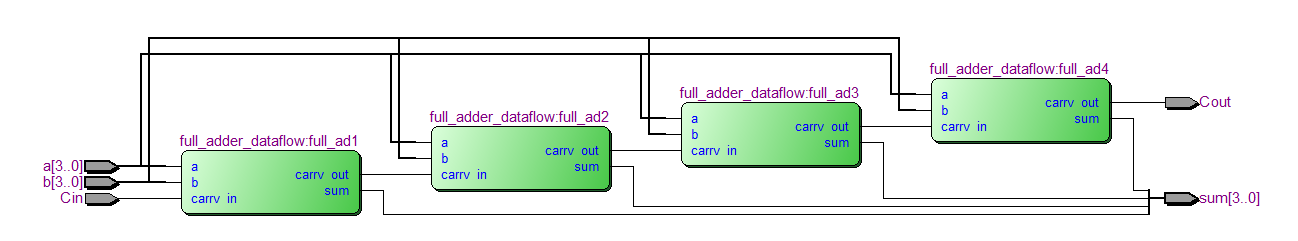
\includegraphics[scale=0.6]{pictures/Oevelse2/four_bit_full_adder_RTLview.jpeg}
\caption{Four bit parallel adder - Structural RTL view}
\label{fig:4bitFaBehavioralRTL}
\end{figure}

	\begin{figure}[H]
		\item[3)]
		Vi starter med at sætte bits til 00001111 samt cin 0 og får det forventede resultat:
		\centering
		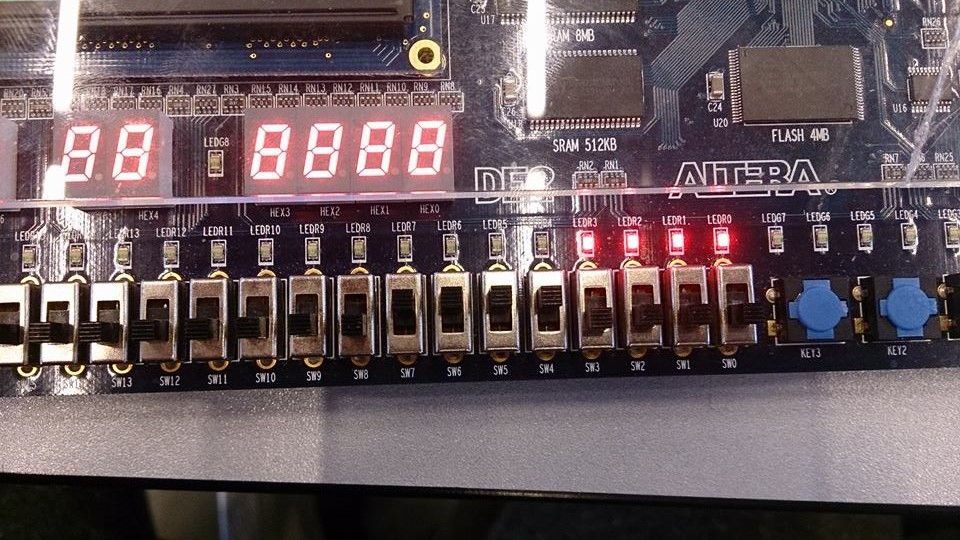
\includegraphics[scale=0.5]{pictures/Oevelse3/00001111_cin0.jpg}
		\caption{Four bit parallel adder - 00001111, cin=0}
		\label{fig:4bitFa00001111cin0}
	\end{figure}

	\begin{figure}[H]
Vi sætter nu bits til 11110000 samt cin 1 og får det forventede resultat:
		\centering
		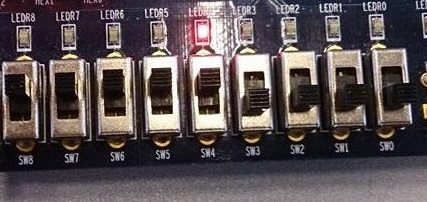
\includegraphics[scale=0.5]{pictures/Oevelse3/11110000_cin1.jpg}
		\caption{Four bit parallel adder - 11110000, cin=1}
		\label{fig:4bitFa11110000cin1}
	\end{figure}


	\begin{figure}[H]
			Vi sætter nu bits til 00010001 samt cin 1 og får det forventede resultat:
			\centering
			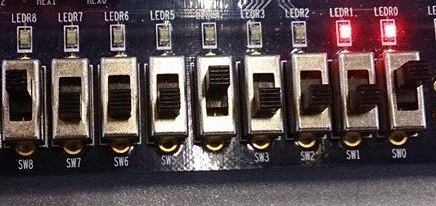
\includegraphics[scale=0.5]{pictures/Oevelse3/00010001_cin1.jpg}
			\caption{Four bit parallel adder - 00010001, cin=1}
			\label{fig:4bitFa00010001cin1}
		\end{figure}
		
\end{enumerate}